\chapter{Estado del arte}
\label{cha:state_of_art}


\section{Tecnologías de contenerización}

Las tecnologías de contenerización se inspiran en el diseño orientado a servicios de aplicaciones. De esta manera, las aplicaciones se descomponen en componentes funcionales o microservicios empaquetados individualmente, junto con todas sus dependencias. Estos componentes, llamados contenedores, pueden implementarse fácilmente en arquitecturas irregulares, simplificando la escalabilidad y actualización de las mismas.

De esta manera, las aplicaciones orientadas a servicios dividen la funcionalidad del sistema en contenedores que se comunican unos con otros a través de interfaces bien definidas. Cada contenedor puede escalar o crecer de manera independiente.

Las aplicaciones que implementan este tipo de diseño no tienen que preocuparse de las especificaciones del sistema anfitrión. En su lugar, cada contenedor debe proporcionar \textit{APIs} consistentes que los clientes puedan usar para acceder al servicio. Estas estrategias permiten a cada componente intercambiarse o actualizarse mientras la \textit{API} lo mantenga.

Algunos de los beneficios del uso de estas tecnologías son:
\begin{itemize}
\item Abstracción del sistema anfitrión donde se ejecutará la aplicación contenerizada mediante interfaces definidas, con independencia de los recursos o arquitecturas del sistema anfitrión.
\item Escalabilidad en pruebas y puesta en producción.
\item Administración simplificada de dependencias y versiones de aplicaciones.
\item Ambientes de ejecución aislados a nivel de proceso.
\item Compartir contenedores evitando la duplicación y ocupando menor espacio en disco.
\end{itemize}

\subsection{Contenedores y Máquinas Virtuales}

Los contenedores se diferencian de las máquinas virtuales en la ubicación de la capa de virtualización y en la forma en que se utilizan los recursos del sistema operativo.

Las máquinas virtuales se basan en un hipervisor que se instala encima del hardware del sistema o del sistema operativo. Luego, las instancias de las máquinas virtuales se pueden aprovisionar a partir de los recursos disponibles en el sistema. De esta manera las máquinas virtuales están completamente aisladas unas de otras y se pueden migrar de un sistema virtualizado a otro sin tener en cuenta el hardware del sistema o los sistemas operativos.

Ahora bien, el entorno de los contenedores está dispuesto de manera diferente. Los contenedores se instalan encima de un sistema operativo anfitrión. Estas instancias de contenedor se pueden aprovisionar a partir de los recursos disponibles del sistema y se pueden implementar las aplicaciones necesarias. De esta manera cada aplicación contenedora comparte el mismo sistema operativo subyacente.

Así, los contenedores se consideran más eficientes que las máquinas virtuales desde el punto de vista de los recursos, puesto que se los recursos adicionales necesarios para cada sistema operativo se eliminan. Por lo tanto, las instancias resultantes son más pequeñas y más rápidas en su creación o migración y un único sistema puede albergar muchos más contenedores que máquinas virtuales.

Sin embargo, hay que tener en cuenta que el sistema operativo único presenta un único punto de error para todos los contenedores que lo utilizan. Por ejemplo, un ataque o bloqueo de malware del sistema operativo anfitrión puede inhabilitar o afectar a todos los contenedores. Además, aunque los contenedores son fáciles de migrar, éstos sólo se pueden migrar a otros servidores con núcleos de sistema operativo compatibles.

\begin{figure}[H]
\centering
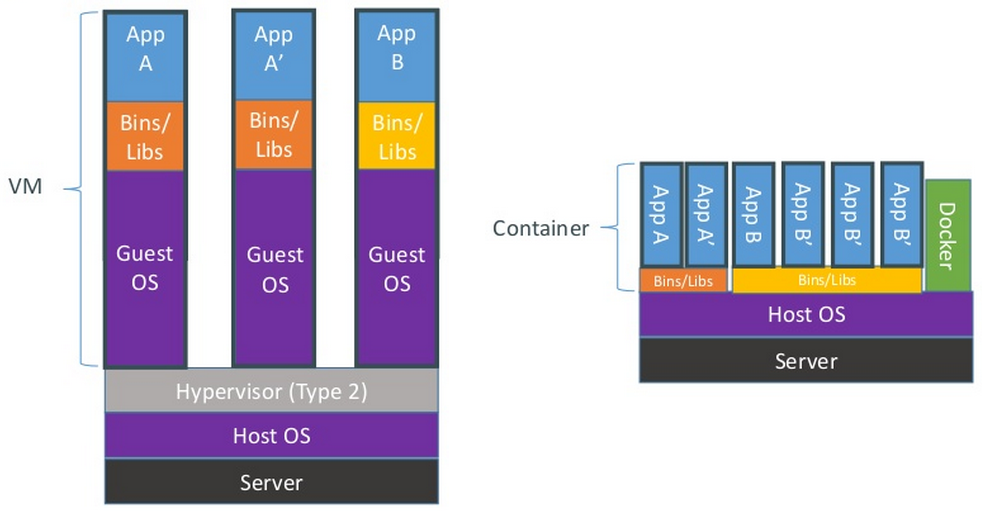
\includegraphics[width=0.7\textwidth]{images/figures/containervsmv.png}
\caption{Diferencia entre máquina virtual y contenedor.\label{fig:figure_placement_example}}
\end{figure}

\subsection{Docker}

En la ejecución de este proyecto se aplicará el uso de Docker\footnotettt{Docker}{https://www.docker.com} como tecnología de contenerización.

\begin{figure}[H]
\centering

\includegraphics[width=0.4\textwidth]{images/figures/docker.png}
\caption{Docker.\label{fig:figure_placement_example}}
\end{figure}

Docker es un software de código abierto introducido como una forma de simplificar las herramientas necesarias para crear y administrar contenedores ligeros y portables, automatizando el despliegue de aplicaciones.

Surgió como un proyecto interno dentro de la empresa dotCloud\footnotettt{dotCloud}{https://www.get.cloud/home.aspx}, por Salomón Hykes, y fue liberado como código abierto en marzo de 2013.

Para su funcionamiento, existen repositorios Docker o registros Docker que contienen imágenes puestas a disposición del público. Las imágenes de Docker son plantillas de solo lectura que consisten en una instantánea de una distribución Linux\footnotettt{Linux}{http://www.linux-es.org} y un conjunto de aplicaciones. Éstas pueden ser públicas o privadas.

Los pasos de configuración se especifican en un fichero de compilación, llamado \kode{Dockerfile}, que describe cómo crear la imagen del contenedor.

\begin{figure}[H]
\centering
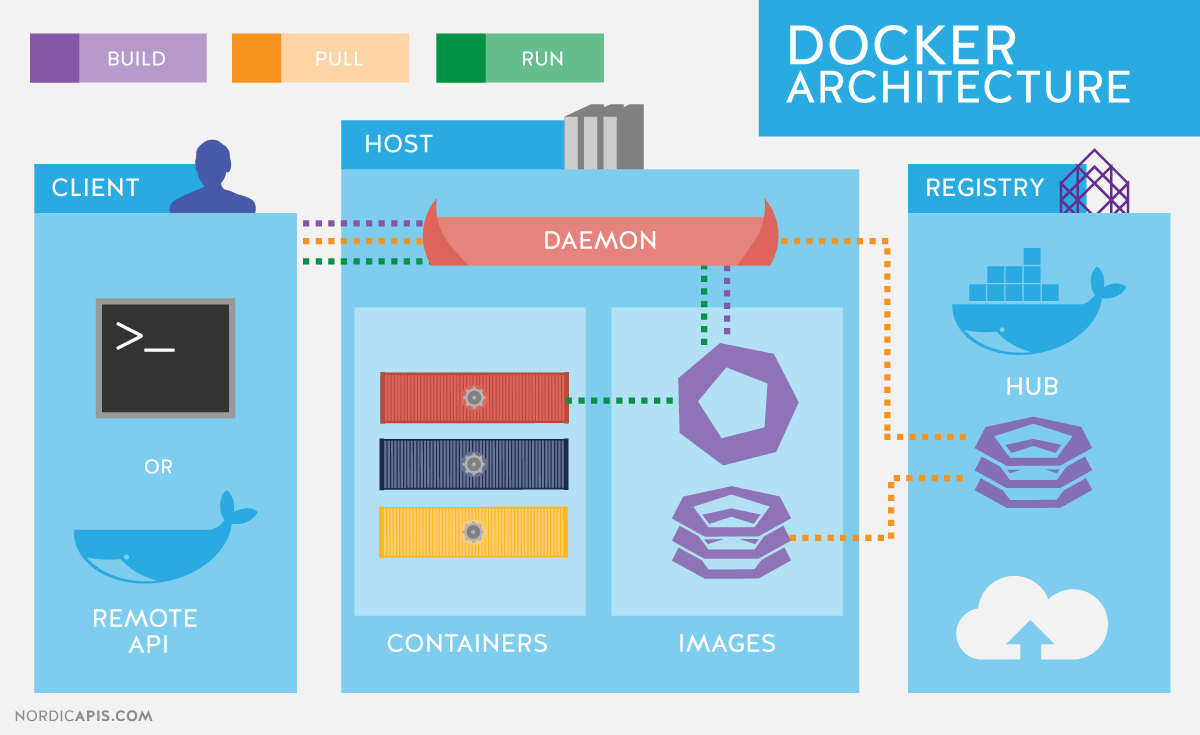
\includegraphics[width=0.7\textwidth]{images/figures/dockerarchitecture.png}
\caption{Arquitectura Docker.\label{fig:figure_placement_example}}
\end{figure}

Cada instalación de Docker incluye un cliente Docker, normalmente una interfaz de línea de comandos. También incluye una \textit{API} remota y un demonio. Tanto el cliente como el demonio pueden compartir un único sistema anfitrión o el demonio puede ejecutarse en un sistema anfitrión remoto. Así, los contenedores Docker son directorios que contienen todo los necesario para que la aplicación se ejecute de forma aislada, incluyendo el sistema operativo y un sistema de ficheros. Esto permite que los contenedores puedan moverse de sistema anfitrión sin riesgo de errores de configuración.

\subsection{Otras tecnologías de contenedores}

Otra tecnología de contenedores es rkt, software de código abierto del equipo que desarrolla CoreOS. 

\begin{figure}[H]
\centering

\includegraphics[width=0.3\textwidth]{images/figures/rkt.png}
\caption{Tecnología de contenedores rkt.\label{fig:figure_placement_example}}
\end{figure}

Este es un gestor de contenedores de última generación para clústeres de Linux. Está diseñado para la seguridad, simplicidad y componibilidad. Así, rkt descubre, verifica, extrae y ejecuta contenedores aislados de aplicaciones que pueden ser conetables. El mismo contenedor puede ser ejecutado con diversos grados de protección, desde el espacio de nombres y el aislamiento de capacidades ligeras y de nivel de sistema operativo hasta la virtualización hadware a nivel de máquina virtual pesada.

La interfaz principal de rkt comprende un solo ejecutable, en lugar de un demonio. Este diseño es aprovechado para integrarse fácilmente con los sistemas de inicio existentes y con entornos de orquestación de clúster avanzados, como Kubernetes. De este modo, se implementa un formato de contenedor moderno, abierto y estándar, el \textit{App Container} (appc)\footnotettt{App Container}{https://coreos.com/rkt/docs/latest/app-container.html}, pero también se puede ejecutar otras imágenes de contenedores, como las creadas con Docker.

\section{Sistemas operativos orientados a contenedores}

Tras el éxito y popularidad de las tecnologías de contenerización han surgido sistemas operativos modernos diseñados para funcionar de manera óptima con un ecosistema de contenedores. Estos sistemas operativos proporcionan la mínima funcionalidad requerida para implementar aplicaciones, junto con propiedades de auto actualización y restablecimiento.

Los sistemas operativos orientados a contenedores han evolucionado el modelo operativo tradicional moviéndose hacia el despliegue de aplicaciones dentro de contenedores frente a la implementación de aplicaciones en la capa de aplicación. De forma más simple, aquí las aplicaciones son binarios autónomos que se pueden mover en su entorno de contenedor.

Esta tecnología también se conoce como la virtualización del sistema operativo en el que su núcleo permite la existencia de múltiples instancias de espacio de usuario aisladas, en lugar de una sola. Estas instancias son los contenedores que pueden parecer y sentirse como un servidor real desde el punto de vista de sus usuarios.

En el desarrollo de este proyecto se utilizará el sistema operativo orientado a contenedores CoreOS\footnotettt{CoreOS}{https://coreos.com}, descrito a continuación.

\subsection{CoreOS}

CoreOS es un sistema operativo ligero de código abierto, de la compañía con el mismo nombre, basado en el núcleo de Linux y lanzado en octubre de 2013. Esta distribución Linux proporciona las características necesarias para ejecutar contenedores con un enfoque práctico para las actualizaciones del sistema operativo. La filosofía de actualización de CoreOS es que su realización frecuente y confiable es fundamental para una buena seguridad. Las actualizaciones se distribuyen como están disponibles y se pueden instalar de forma inmediata y automática.  

\begin{figure}[H]
\centering

\includegraphics[width=0.4\textwidth]{images/figures/coreos.png}
\caption{CoreOS.\label{fig:figure_placement_example}}
\end{figure}

CoreOS está diseñado para implementar una aplicación distribuida en un clúster de nodos. Así, se encarga de proporcionar la infraestructura necesaria para los despliegues en clúster, automatización, seguridad, fiabilidad y escalabilidad. CoreOS ofrece las funcionalidades mínimas necesarias para la implementación de aplicaciones dentro de contenedores de software, junto con mecanismos incorporados para el descubrimiento de servicios y el intercambio de configuración.

CoreOS es una bifurcación de Chrome OS\footnotettt{Chrome OS}{https://sites.google.com/site/chromeoslinux}, sistema operativo basado en web, de la compañía Google\footnotettt{Google}{https://www.google.com/about/company}, por medio de la utilización de su kit de desarrollo de software (\textit{SDK}). Está disponible gratuitamente a través de Chromium OS\footnotettt{Chromium OS}{https://www.chromium.org/chromium-os} como base, al tiempo que añade nuevas funcionalidades y personalización para soportar el hardware, utilizando servidores.

CoreOS no proporciona un gestor de paquetes, por lo que requiere que todas las aplicaciones se ejecuten dentro de sus contenedores. Para ello utiliza Docker y contenedores Linux subyacentes de virtualización, a nivel de sistema operativo, para la ejecución de múltiples sistemas Linux aislados en un único sistema anfitrión de control, que sería la instancia CoreOS. De esa manera, la partición de recursos se lleva a cabo a través de múltiples instancias de espacios de usuario aisladas, en lugar de utilizar un hipervisor y una máquina virtual. Este enfoque se basa en cgroups, funcionalidad del núcleo de Linux que ofrece aislamiento del espacio de nombres y habilidades para limitar, contabilizar y aislar el uso de los recursos de un grupo de procesos.

Para mayor seguridad y fiabilidad en actualizaciones, CoreOS emplea \textit{FastPatch} como esquema de doble partición para su sola lectura del sistema de archivos raíz, lo que significa que las actualizaciones del sistema operativo se llevan a cabo en su totalidad y se instalan en una partición raíz secundaria pasiva, que se activa al reiniciar o realizando una ejecución del núcleo (\textit{kexec}).

El sistema de distribución de actualizaciones de CoreOS se basa en el proyecto de código abierto de Google Omaha\footnotettt{Google Omaha}{https://github.com/google/omaha}, que proporciona un mecanismo para el despliegue de actualizaciones y el protocolo subyacente petición-respuesta sobre la base de \textit{XML}.

\begin{figure}[H]
\centering
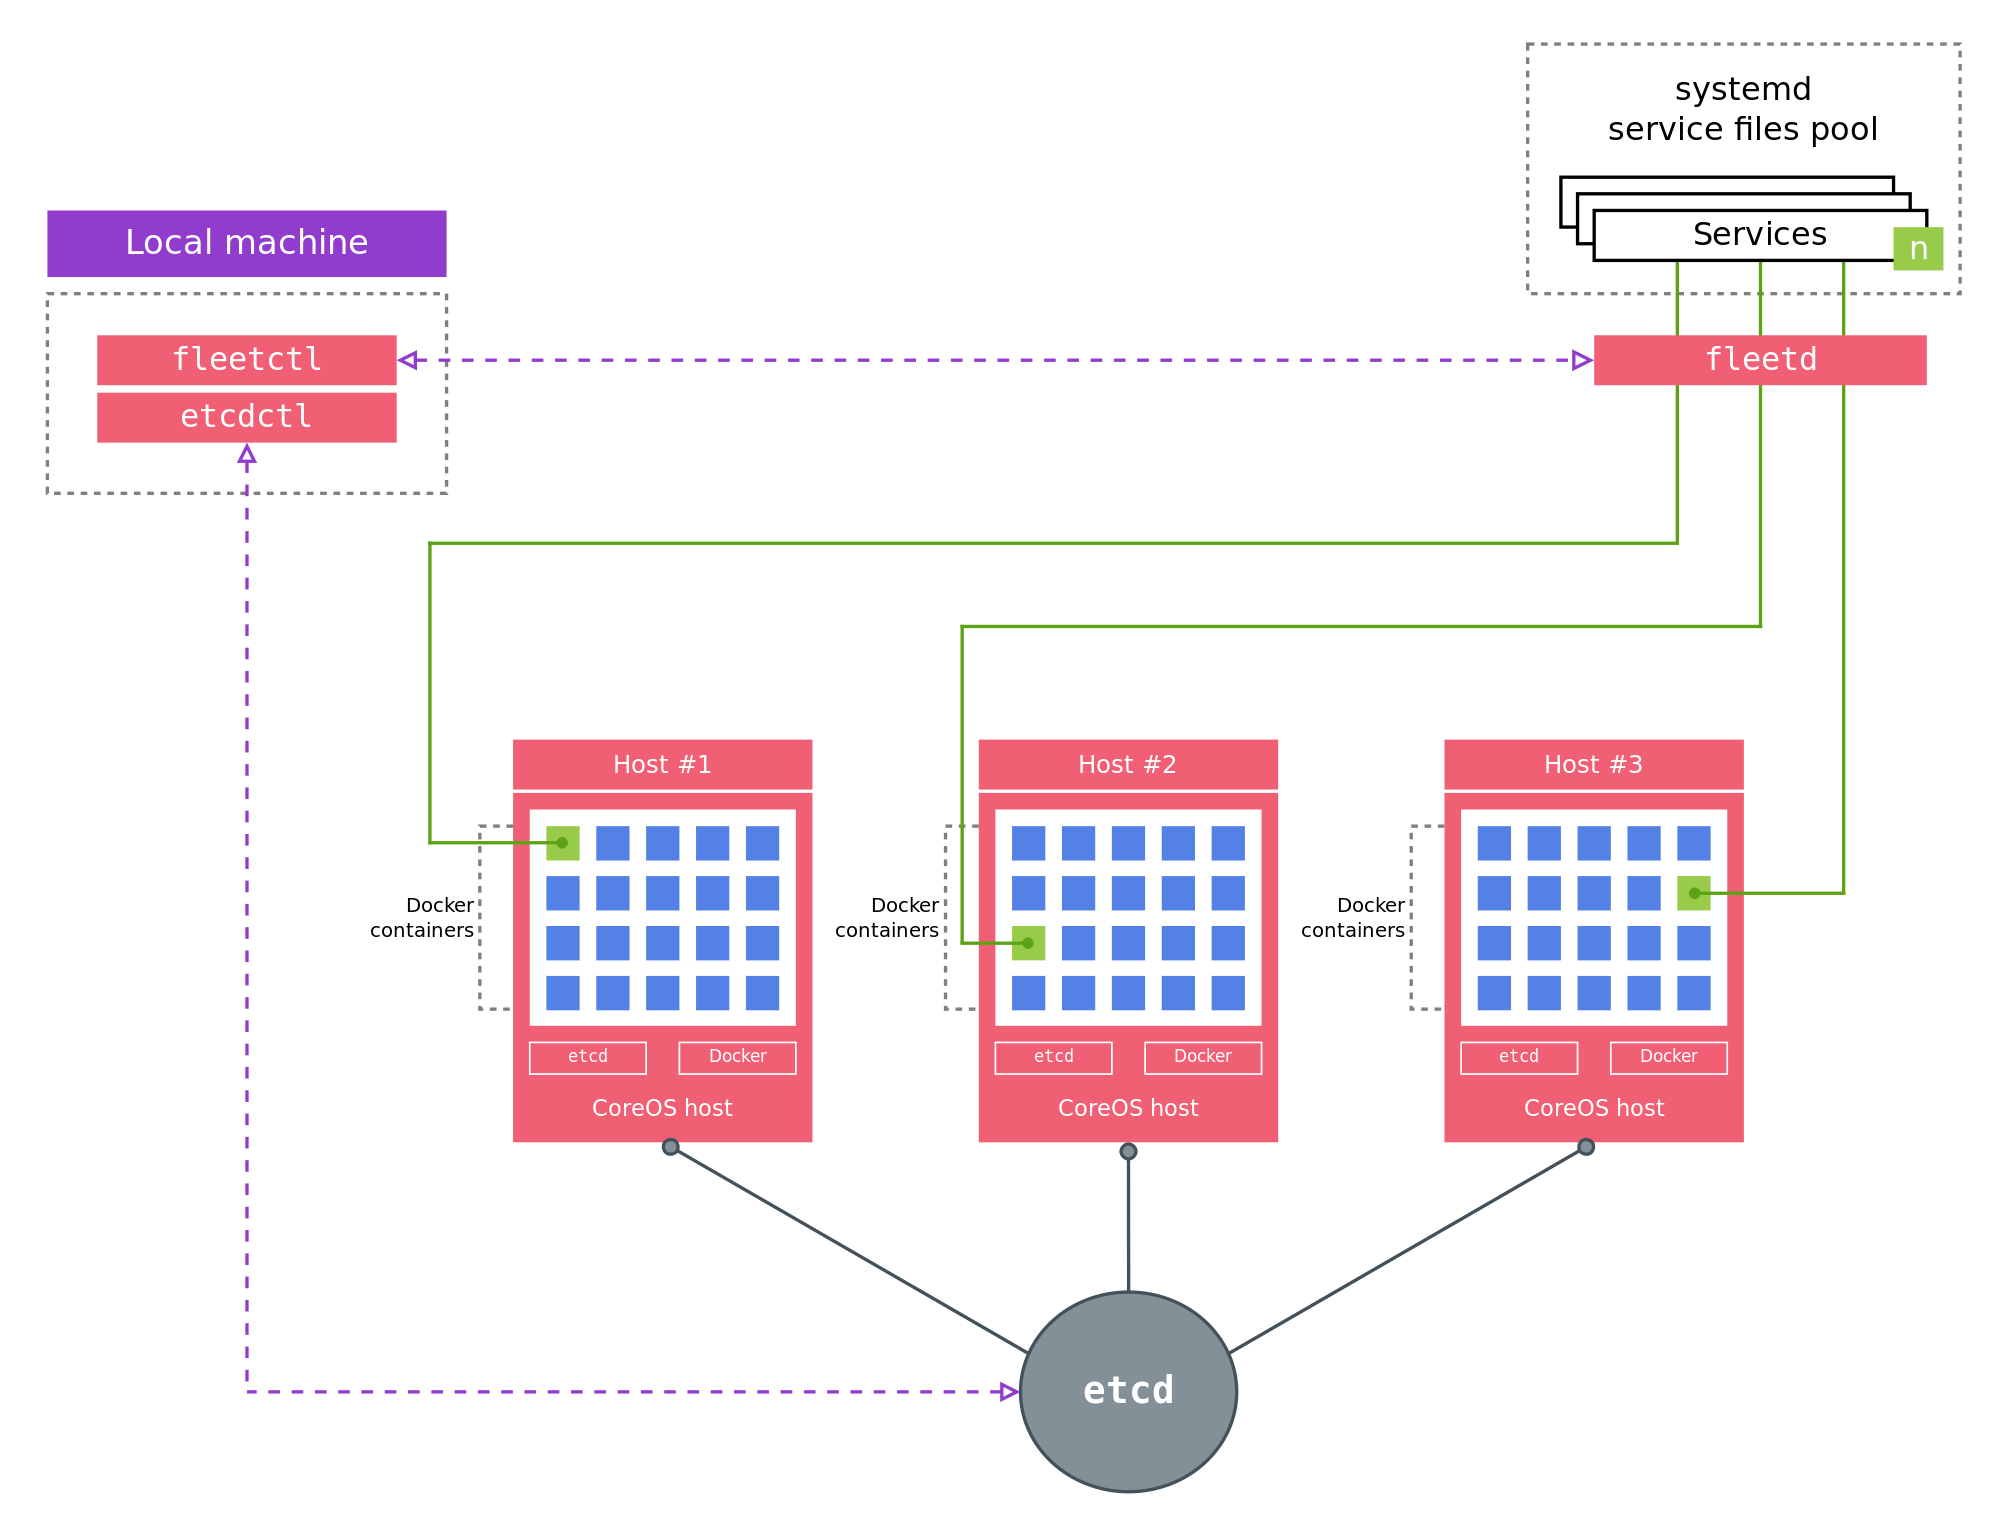
\includegraphics[width=0.8\textwidth]{images/figures/coreosarchitecture.png}
\caption{Arquitectura CoreOS.\label{fig:figure_placement_example}}
\end{figure}

Los principales componentes de CoreOS son su núcleo, systemd\footnotettt{systemd}{https://coreos.com/docs/launching-containers/launching/getting-started-with-systemd}, etcd\footnotettt{etcd}{https://coreos.com/etcd}, fleet\footnotettt{fleet}{https://coreos.com/fleet}, flannel\footnotettt{flannel}{https://coreos.com/flannel/docs/latest/flannel-config.html} y rkt\footnotettt{rkt}{https://coreos.com/rkt}. En cuanto a su ecosistema se tiene Docker y Kubernetes\footnotettt{Kubernetes}{http://kubernetes.io}, este último explicado en el siguiente capítulo.

Sus propiedades claves a destacar son las siguientes:

\begin{itemize}
\item El núcleo es muy pequeño y rápido para arrancar.
\item El sistema operativo base y todos los servicios son de código abierto.
\item Los servicios también se pueden usar de manera independiente en sistemas que no son CoreOS.
\item El sistema operativo no proporciona gestor de paquetes. Las bibliotecas y los paquetes forman parte de la aplicación desarrollada mediante contenedores.
\item Permite clústeres seguros de muchos servidores que pueden utilizarse para el despliegue de aplicaciones distribuidas.
\item Cada proceso es administrado por el servicio systemd.
\item etcd, fleet y flannel son unidades de control que se ejecutan como procesos del núcleo.
\item Los canales de lanzamiento CoreOS (estable, beta y alfa) se utilizan para controlar el ciclo de lanzamiento.
\item Los productos comerciales incluyen: el servicio CoreUpdate\footnotettt{CoreUpdate}{https://coreos.com/products/coreupdate}, un panel de control web para la gestión de actualizaciones del clúster, Quay entreprise\footnotettt{Quay entreprise}{https://quay.io/enterprise}, repositorios de contenedores, y Tectonic\footnotettt{Tectonic}{https://tectonic.com}, que conecta el uso de CoreOS junto con Kubernetes, explicado con mayor detalle en el siguiente apartado.
\item Actualmente se ejecuta en procesadores x86.
\end{itemize}

Entre sus ventajas significativas cabe destacar:

\begin{itemize}
\item La función de actualización automática del núcleo lo protege de las vulnerabilidades de seguridad.
\item Utiliza muy poca memoria respecto a otras distribuciones.
\item La gestión de las máquinas CoreOS se realiza en el nivel de clúster en lugar de nivel de máquina individual.
\item Es compatible con todos los principales proveedores de nube, como Amazon Web Services\footnotettt{AWS}{https://aws.amazon.com/es}, GCE\footnotettt{GCE}{https://cloud.google.com/compute/docs}, Azure\footnotettt{Azure}{https://azure.microsoft.com/es-es} y DigitalOcean\footnotettt{DigitalOcean}{https://www.digitalocean.com}.
\item La mayoría de los componentes de CoreOS son de código abierto y el cliente puede elegir la combinación de herramientas necesaria para su aplicación específica.
\end{itemize}

A continuación se detallan los microservicios de CoreOS a utilizar en el desarrollo de este proyecto.

\subsubsection{Systemd}

Systemd es un sistema de inicio que CoreOS utiliza para iniciar, detener y administrar procesos. Los sistemas más comunes de inicio utilizados en Unix\footnotettt{Unix}{http://www.opengroup.org/unix} son el propio systemd en CoreOS y RedHat\footnotettt{RedHat}{https://www.redhat.com/es}, Upstart\footnotettt{Upstart}{http://upstart.ubuntu.com/getting-started.html} en Ubuntu y Supervisord\footnotettt{Supervisord}{http://supervisord.org} en el mundo Python\footnotettt{Python}{https://www.python.org}.

Un sistema de inicio común tiene las funciones de ser el primer proceso en comenzar, controlar el orden y ejecución de todos los procesos de usuario, ocuparse de reiniciar procesos, si mueren o cuelgan, y de la propiedad del proceso y sus recursos.

Específicamente, cada proceso en systemd se ejecuta en un \textit{cgroup}, característica del núcleo de Linux que limita, contabiliza y aísla el uso de recursos de una colección de procesos. Si el servicio systemd se cancela, todos los procesos asociados con el servicio, incluidos los procesos bifurcados, se eliminan. Si se ejecuta un contenedor en systemd se puede controlar el uso de recursos, incluso si el contenedor contiene varios procesos.
 
Las unidades systemd se ejecutan y controlan en una sola máquina. Éstas describen una tarea en particular junto con sus dependencias y orden de ejecución. Algunas unidades se inician en el sistema de forma predeterminada y otras por usuarios. Las unidades iniciadas por el sistema están en \kode{/usr/lib64/systemd/system} y las iniciadas por el usuario en \kode{/etc/systemd/system}.

La interfaz de línea de comandos (\textit{CLI}) systemctl puede utilizarse para controlar unidades systemd.

Algunos tipos de unidad systemd son \textit{service}, \textit{socket}, \textit{target}, \textit{mount} y \textit{timer}. El tipo más común es \textit{service} y se utiliza para definir un servicio con sus dependencias. El tipo \textit{socket} se utiliza para exponer los servicios al mundo externo. Por ejemplo, \textit{docker.service} expone la conectividad externa al motor Docker a través de \textit{docker.socket}. Los \textit{sockets} también se pueden utilizar para exportar registros a máquinas externas. Por su parte, la unidad \textit{target} se utiliza para agrupar unidades relacionadas para que puedan ser iniciadas conjuntamente y la unidad \textit{mount} para montar discos en el sistema de archivos. Por último, las unidades timer se inician periódicamente en función del intervalo especificado.

Una unidad systemd puede ser creada a partir de una plantilla y ésta ser utilizada para instanciar varias unidades.

También existe el concepto de unidades sueltas, útiles para cambiar las propiedades de la unidad del sistema en tiempo de ejecución. Así como las unidades de red.

\subsubsection{Etcd}

Etcd es un sistema de almacenamiento de pares clave-valor distribuido utilizado por todas las máquinas del clúster CoreOS para leer, escribir e intercambiar datos. Etcd utiliza el algoritmo Raft para mantener un clúster en alta disponibilidad. Además, se utiliza para compartir la configuración y los datos de monitorización en los equipos CoreOS y para realizar el descubrimiento del servicio. Todos los demás servicios de CoreOS usan etcd como una base de datos distribuida. 

La utilidad etcdctl es la interfaz \textit{CLI} para etcd.

Los parámetros de configuración de etcd se pueden usar para modificar propiedades de un sólo miembro etcd o de todo el clúster. Estas opciones se clasifican entre las siguientes categorías:

\begin{itemize}
\item Miembro: Nombre, directorio de datos e intervalo de latido.
\item Clúster: Señal de descubrimiento y nodos de clúster iniciales.
\item Proxy: Activado/Desactivado e intervalos.
\item Seguridad: Certificado y clave.
\item Registro: Habilitar/Deshabilitar registro y niveles de registro.
\end{itemize}

Las operaciones principales que se pueden hacer usando etcd son:

\begin{itemize}
\item Establecer, obtener y eliminar operaciones de un par clave-valor.
\item Establecer una clave que expire automáticamente tras un tiempo definido. 
\item Establecer una clave basada en la comprobación de una condición atómica.
\item Claves ocultas.
\item Observación y espera ante cambios en claves.
\item Creación de claves bajo petición.
\end{itemize}

\subsubsection{Fleet} \label{sssec:fleet}

El servicio fleet es un gestor o planificador que controla la creación de servicios a nivel de clúster. Mientras que systemd actua como sistema de inicio para un nodo, fleet es el sistema de inicio para el clúster y usa el servicio etcd para la comunicación entre nodos.

Al tratarse de una herramienta para la orquestación de contenedores será descrita con mayor detalle en la sección \ref{sec:herramientas}.

\subsubsection{Flannel}

Flannel utiliza una red de superposición para permitir que contenedores, a través de diferentes anfitriones, se comuniquen entre sí. Flannel no es parte de la imagen básica de CoreOS para poder mantener el tamaño de la imagen CoreOS mínimo. Así, cuando se inicia flannel su imagen se recupera del repositorio de imágenes de contenedor. 

El demonio Docker se inicia, normalmente, después del servicio flannel para que los contenedores puedan obtener la dirección IP asignada por flannel. Esto representa un problema puesto que Docker es necesario para descargar la imagen de flannel. CoreOS ha resuelto este problema ejecutando un servicio Docker maestro cuyo único propósito es descargar el contenedor flannel.

Entre sus características cabe destacar que flannel se ejecuta sin un servidor central y utiliza etcd para la comunicación entre los nodos. Como parte del inicio de flannel, se necesita proporcionar un archivo de configuración que contenga la subred IP que se utilizará para el clúster, así como el protocolo en uso.

Cada nodo del clúster solicita un rango de direcciones IP para los contenedores creados en ese anfitrión y lo registra con etcd. Como cada nodo del clúster conoce el rango de direcciones IP asignado para cada otro nodo, sabe cómo llegar a los contenedores creados en cualquier nodo del clúster. Cuando se crean contenedores, los contenedores obtienen una dirección IP dentro del rango asignado al nodo y si necesitan comunicarse a través de anfitriones, flannel hace la encapsulación basada en el protocolo elegido. Así, flannel en el nodo de destino desencapsula el paquete y lo entrega al contenedor.

Al no utilizar la asignación basada en puertos para hablar a través de los contenedores, flannel simplifica la comunicación contenedor a contenedor.

Las razones por las que se necesita crear redes de contenedores son:
\begin{itemize}
\item Los contenedores necesitan comunicarse con el mundo exterior.
\item Los contenedores deben ser accesibles desde el mundo exterior para que éste pueda utilizar los servicios que proporcionan.
\item Los contenedores necesitan comunicarse con la máquina anfitriona.
\item Debería haber conectividad entre contenedores en el mismo anfitrión y entre anfitriones.
\end{itemize}

\subsubsection{Confd}

La herramienta confd está diseñada para ver cambios en los almacenes distribuidos de clave-valor. Se ejecuta dentro de un contenedor Docker y se utiliza para activar modificaciones de configuración y recargas de servicio.

Esta herramienta de gestión de configuración está construida en la parte superior de etcd. Así, confd puede ver ciertas claves en etcd y actualizar los archivos de configuración relacionados a ellas tan pronto como ésta cambie. Luego, confd puede volver a cargar o reiniciar las aplicaciones relacionadas con los archivos de configuración actualizados. Esto le permite automatizar los cambios de configuración a todos los servidores del clúster y asegura que todos los servicios están siempre buscando la última configuración.

En la siguiente imagen se aprecia un ejemplo de uso y funcionamiento común compuesto por los siguientes elementos: 
\begin{itemize}
\item Un contenedor apache, representando a una aplicación, que se registra con etcd permitiendo que todos los contenedores disponibles sean descubiertos. 
\item Un volumen de datos en el que confd puede escribir su configuración.
\item Un contenedor que ejecuta confd y vigila los cambios en etcd para construir un archivo de configuración \textit{ngnix} usado, a su vez, para equilibrar la carga entre los contenedores disponibles.
\item Un contenedor \textit{nginx} que obtiene la configuración a partir del volumen compartido.
\end{itemize}

Cuando esté funcionando se podrán agregar nuevos contenedores de apache que, a su vez, se asignen automáticamente al equilibrador de carga.

\begin{figure}[H]
\centering
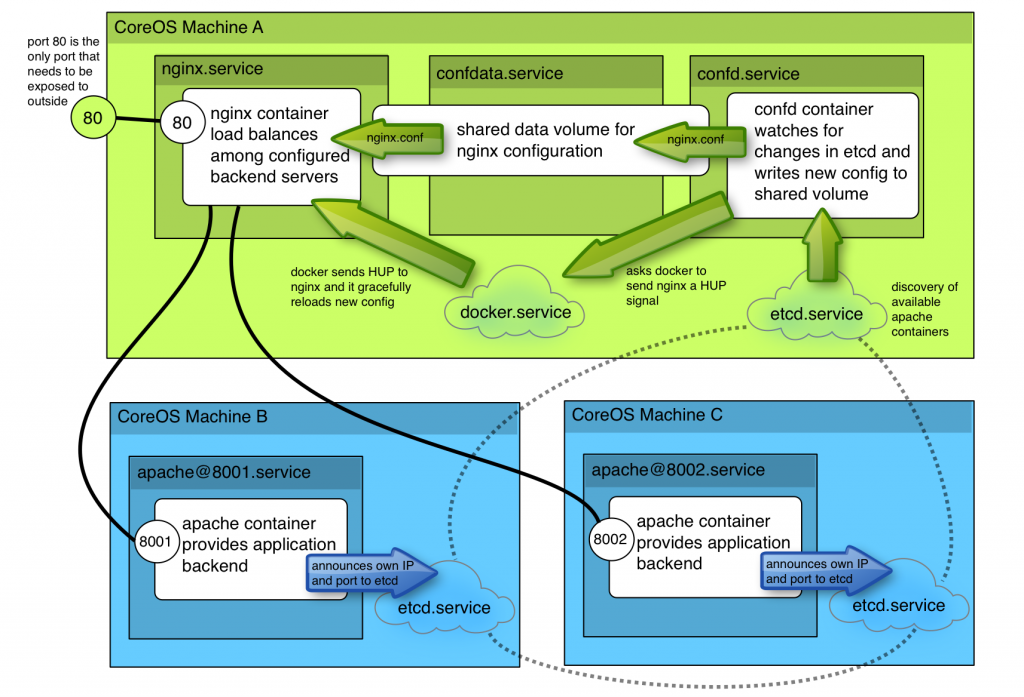
\includegraphics[width=0.8\textwidth]{images/figures/loadbalancerconfd.png}
\caption{Balanceador de carga con CoreOS, confd y \textit{nginx}.\label{fig:figure_placement_example}}
\end{figure}

\subsection{Otros}

Aparte de CoreOS, los otros dos principales sistemas operativos orientados a contenedores son  Red Hat Enterprise Linux (RHEL) Project Atomic\footnotettt{Project Atomic}{https://www.projectatomic.io} y Snappy Ubuntu Core\footnotettt{Snappy Ubuntu Core}{https://developer.ubuntu.com/en/snappy}.

Project Atomic facilita la arquitectura centrada en la aplicación al proporcionar una solución para desplegar aplicaciones contenedoras de forma rápida y confiable. La actualización atómica y la reversión de aplicaciones y anfitriones permiten la implementación de pequeñas mejoras frecuentes. Concretamente, RHEL Project Atomic, lanzado en 2014, es un sistema operativo ligero montado a partir del contenido del RMP Package Manager\footnotettt{RMP Package Manager}{http://rpm.org}. Se trata de una variante optimizada de RHEL 7\footnotettt{RHEL 7}{https://access.redhat.com/documentation/en-US/Red\_Hat\_Enterprise\_Linux/7/html/7.0\_Release\_Notes} para ejecutar contenedores Linux.

\begin{figure}[H]
\centering

\includegraphics[width=0.2\textwidth]{images/figures/projectatomic.png}
\caption{Project Atomic.\label{fig:figure_placement_example}}
\end{figure}

Por su parte Snappy Ubuntu Core, lanzado en 2014, es un sistema operativo que usa una imagen de servidor mínima con las mismas bibliotecas que el sistema operativo Ubuntu\footnotettt{Ubuntu}{https://www.ubuntu.com} actual, pero las aplicaciones se proporcionan a través de un mecanismo más simple. Su enfoque ágil es más rápido, más fiable y permite ofrecer mayores garantías de seguridad para aplicaciones y usuarios. Las aplicaciones Snappy y Ubuntu Core se pueden actualizar de forma atómica y revertirse si es necesario, pensando para contenedores.

\begin{figure}[H]
\centering

\includegraphics[width=0.2\textwidth]{images/figures/snappyubuntu.png}
\caption{Snappy Ubuntu.\label{fig:figure_placement_example}}
\end{figure}

\section{Herramientas para la orquestación de contenedores} \label{sec:herramientas}

Un sistema de orquestación de contenedores trata el hardware dispar de la infraestructura como una colección y lo representa para la aplicación como un único recurso. También, programa los contenedores basándose en las restricciones de los usuarios y utiliza la infraestructura de la manera más eficiente posible, escalando los contenedores dinámicamente y manteniendo los servicios en alta disponibilidad.

Las principales herramientas para la orquestación de contenedores en la actualidad son, por un lado, Fleet y Kubernetes y, por otro, Docker Swarm\footnotettt{Docker Swarm}{https://www.docker.com/products/docker-swarm} y Apache Mesos\footnotettt{Apache Mesos}{http://mesos.apache.org}.

A continuación se describen, con especial relevancia, los dos primeros.

\subsection{Fleet}

Como se vió en la sección \ref{sssec:fleet}, fleet es un componente de CoreOS que controla la creación de servicios a nivel de clúster.

Fleet utiliza el modelo maestro-esclavo, donde el motor fleet desempeña el papel de maestro y el agente fleet representa el papel de esclavo.

El motor es reponsable de programar las unidades fleet y el agente de ejecutarlas y divulgar su estado al motor. Un motor maestro es elegido entre el núcleo de CoreOS utilizando etcd. Cuando el usuario inicia un servicio fleet cada agente ofrece ese servicio. Fleet utiliza un algoritmo de programación de carga mínima muy simple para programar la unidad en el nodo apropiado. Las unidades fleet también constan de metadatos para controlar dónde se ejecuta la unidad con respecto a la propiedad del nodo, así como la base de otros servicios que se ejecutan en ese nodo en particular. El agente procesa la unidad y la ofrece a systemd para su ejecución. Si un nodo muere se elige un nuevo motor y las unidades de programa en ese nodo se reprograman en un nuevo nodo. 

Systemd proporciona alta disponibilidad a nivel de nodo, mientras que fleet lo hace a nivel de clúster. Así, fleet se utiliza principalmente para la orquestación de servicios críticos del sistema, usando systemd. 

Otras soluciones de orquestación, como Kubernetes, se usan para la orquestación de servicios de aplicación en contenedores. No obstante, fleet se puede utilizar para la orquestación de pequeñas aplicaciones.

Fleet soporta especificadores de unidades y plantillas similares a systemd. Un especificador de unidad le proporciona accesos directos dentro de un archivo de servicio y las plantillas proporcionan archivos de servicio reutilizables.

Los metadatos se pueden utilizar en archivos de servicio fleet para controlar la programación y las opciones X-Fleet se usan para especificar restricciones al programar el servicio. Entre las disponibles se encuentran:
\begin{itemize}
\item \textit{MachineMetaData}: El servicio se programa basado en metadatos coincidentes.
\item \textit{MachineId}: El servicio se programa basado en el \textit{MachineId} especificado.
\item \textit{MachineOf}: El servicio se programa basado en otros servicios que se ejecutan en el mismo nodo. Esto se usa para programar servicios estrechamente acoplados en el mismo nodo.
\item \textit{Conflict}: Esta opción se utiliza para evitar el lanzamiento de servicios en conflicto en el mismo nodo.
\item \textit{Global}: El mismo servicio se programa en todos los nodos del clúster.
\end{itemize}

\subsection{Kubernetes}

Kubernetes es una plataforma de código abierto para la orquestación de contenedores, iniciada por Google.

\begin{figure}[H]
\centering

\includegraphics[width=0.5\textwidth]{images/figures/kubernetes.png}
\caption{Kubernetes.\label{fig:figure_placement_example}}
\end{figure}

La unidad más pequeña en Kubernetes es un \textit{pod}. Los \textit{pods} son un conjunto de contenedores que se encuentran juntos en un único nodo, trabajando estrechamente entre sí. Todos los contenedores de un \textit{pod} comparten el espacio de nombres \textit{IPC}, de red, \textit{UTS} y \textit{PID}. Al compartir el espacio de nombres \textit{IPC}, pueden utilizar dichos mecanismos para comunicarse entre sí. Compartiendo el espacio de nombres de red, los contenedores pueden utilizar sockets para comunicarse entre sí. Cada \textit{pod} tiene una dirección IP y todos los contenedores de ese \textit{pod} la comparten. Además, al compartir el espacio de nombres \textit{UTS}, los volúmenes se pueden montar en un \textit{pod} para que todos los contenedores los vean.

Los \textit{pods} pueden hablar entre sí a través de los nodos utilizando diferentes técnicas como el enrutamiento basado en la nube, Flannel, Weave\footnotettt{Weave}{https://developers.google.com/weave}, Calico\footnotettt{Calico}{https://www.projectcalico.org/learn} y otros.

Los servicios son una abstracción de Kubernetes para combinar lógicamente los \textit{pods} que proporcionan una funcionalidad similar. También se encarga de equilibrar la carga de múltiples \textit{pods}. Los servicios deben ser descubiertos internamente o externamente según su tipo.

Para el descubrimiento de servicio interno, Kubernetes ofrece dos opciones:
\begin{itemize}
\item Variable de entorno: Cuando se crea un nuevo \textit{pod} se pueden importar variables de entorno de servicios antiguos, permitiendo a los servicios comunicarse entre sí.
\item \textit{DNS}: Todos los servicios se registran en el servicio \textit{DNS}, kube-dns\footnotettt{kube-dns}{http://kubernetes.io/docs/admin/dns}, de manera que los nuevos servicios pueden encontrar y comunicarse con otros servicios.
\end{itemize}

Para el descubrimiento de servicio externo, Kubernetes ofrece dos opciones:
\begin{itemize}
\item \textit{NodePort}: Kubernetes expone el servicio a través de puertos especiales (30000-32767) de la dirección IP del nodo.
\item \textit{Loadbalancer}: Kubernetes interactúa con el proveedor de la nube para crear un equilibrador de carga que redirige el tráfico a los \textit{pods}.
\end{itemize}

Kubernetes sigue la arquitectura maestro-esclavo. Los componentes de Kubernetes se pueden dividir entre los que manejan un nodo individual y los que son parte del plano de control. El maestro es la principal unidad de control del cluster que gestiona su carga de trabajo y dirige la comunicación a través del sistema. El plano de control de Kubernetes consta de varios componentes, cada uno con su propio proceso, que puede ejecutarse tanto en un único nodo maestro como en múltiples maestros que soporten clústeres de alta disponibilidad.

Esta herramienta se compone de múltiples servicios como el servidor kubelet\footnotettt{kubelet}{https://coreos.com/blog/introducing-the-kubelet-in-coreos}, el servidor \textit{API}, el planificador y el controlador de replicación, todos ellos funcionando como unidades fleet. Los tres últimos son ejecutados por los nodos maestros. Los nodos esclavos, en cambio, manejan los servicios críticos como kubelet y kube-proxy\footnotettt{kube-proxy}{http://kubernetes.io/docs/admin/kube-proxy}.

La interacción del usuario con Kubernetes se realiza a través de kubectl, que utiliza la \textit{API} estándar. El servidor \textit{API} sirve a la \textit{API} estándar utilizando \textit{JSON} sobre \textit{HTTP}, proporcionando tanto la interfaz interna como externa a Kubernetes. Así, el servidor \textit{API} procesa y valida las peticiones \textit{REST} y actualiza el estado de los objetos \textit{API} en etcd, permitiendo a los clientes configurar cargas de trabajo y contenedores a través de nodos \textit{Worker} o \textit{Minion}, que son los nodos esclavo. 

El planificador es el componente conectable que selecciona en qué nodo debería ejecutarse un \textit{pod} no programado basado en la disponibilidad de recursos y las cargas de trabajo existentes asignadas a través de los servidores.


El controlador de replicación es necesario para mantener la alta disponibilidad de \textit{pods} y crear varias instancias como se especifica en su manifiesto. Los controladores se comunican con el servidor de la API para crear, actualizar y eliminar los recursos que administran. 

El nodo \textit{Worker} o \textit{Minion} es la única máquina virtual donde se despliegan contenedores. Cada nodo del clúster debe ejecutar el contenedor junto con los siguientes componentes, para la comunicación con el maestro y configuración de la red de contenedores:
\begin{itemize}
\item Etcd es utilizado como un repositorio de datos compartidos para que todos los nodos se comuniquen entre sí.
\item \textit{DNS} se utiliza para el descubrimiento del servicio.
\item Kubelet es responsable del estado de ejecución de cada nodo. Se ocupa de iniciar, detener y mantener los contenedores de aplicaciones según lo indicado por el plano de control. El servidor \textit{API} del nodo maestro se comunica con el servicio kubelet de cada nodo esclavo para proporcionar los \textit{pods}. Kubelet monitorea el estado de un \textit{pod} y si no está en el estado deseado, el \textit{pod} será redistribuido al mismo nodo. El estado del nodo se retransmite cada pocos segundos mediante mensajes de latido al maestro. Una vez que el maestro detecta un fallo de nodo, el controlador de replicación observa este cambio de estado y lanza \textit{pods} en otros nodos saludables.
\item Kube-proxy se ocupa de la redirección de servicios y el equilibrio de carga del tráfico en los \textit{pods}. Se trata de una implementación de un proxy de red y un equilibrador de carga, soportando la abstracción de servicios junto con otras operaciones de red. Es responsable de enrutar el tráfico al contenedor apropiado según la IP y número de puerto de la solicitud entrante.
\item CAdvisor\footnotettt{CAdvisor}{https://github.com/google/cadvisor} es un agente que monitorea y recopila el uso de recursos y métricas de rendimiento como la \textit{CPU}, la memoria, el uso de archivos y las redes de contenedores en cada nodo.
\end{itemize}

\begin{figure}[H]
\centering
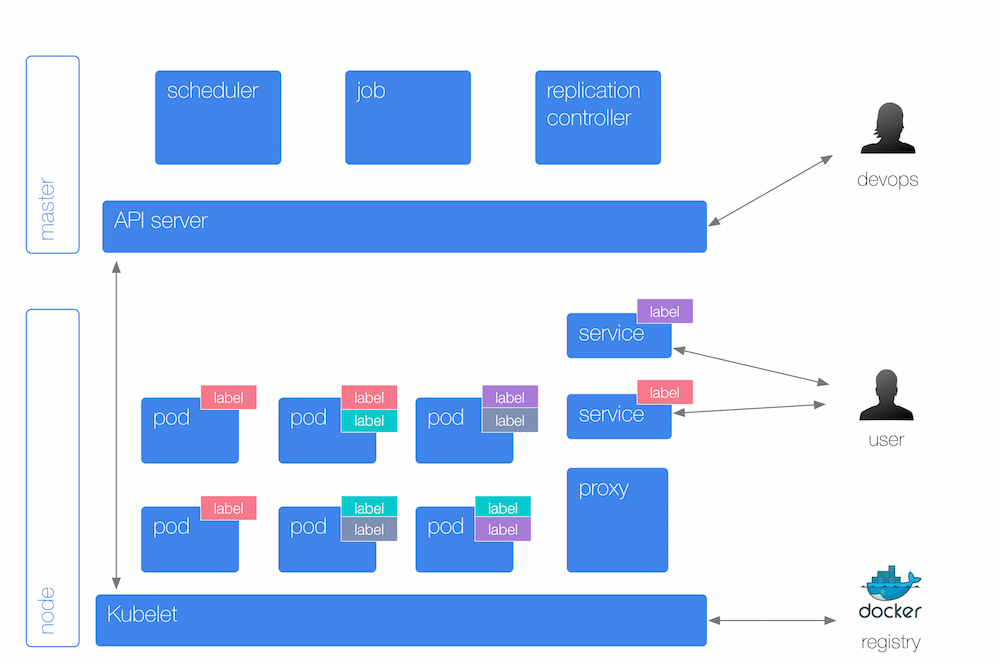
\includegraphics[width=0.8\textwidth]{images/figures/kubernetesarchitecture.png}
\caption{Arquitectura Kubernetes.\label{fig:figure_placement_example}}
\end{figure}

\subsection{Otros}

Docker Swarm es la solución de orquestación nativa de Docker. Con su uso se administra el clúster como sola entidad en lugar de administrar nodos Docker individuales. 

Esta herramienta tiene un planificador integrado que decide la ubicación de los contenedores en el clúster y utiliza restricciones y afinidades específicas del usuario para decidir esa ubicación. En su arquitectura existe un maestro que se encarga de la planificación de contenedores Docker basado en el algoritmo planificador, restricciones y afinidades. Para proporcionar alta disponibilidad se pueden ejecutar múltiples maestros en paralelo, distribuyendo las cargas de trabajo uniformemente. Por su parte, los agentes se ejecutan en cada nodo y se comunican con el maestro a partir del descubrimiento, necesario porque se ejecutan en diferentes nodos y no son iniciados por él.

\begin{figure}[H]
\centering
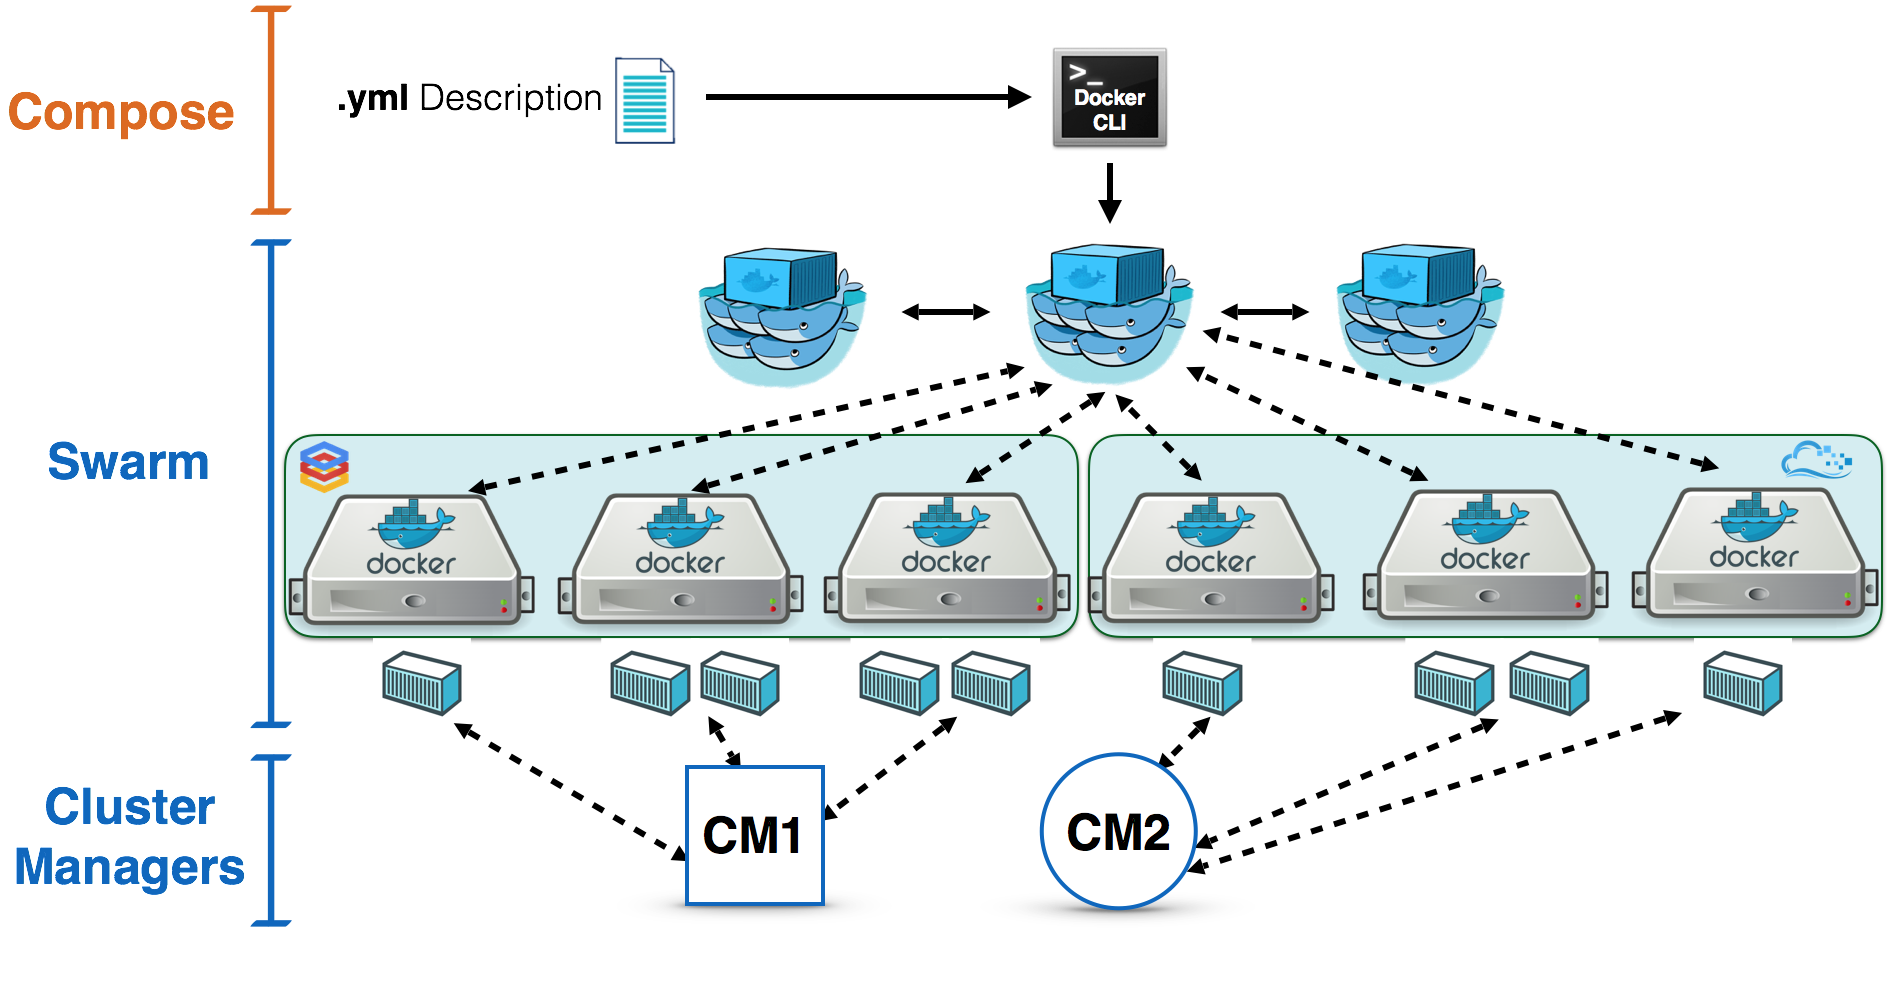
\includegraphics[width=0.7\textwidth]{images/figures/dockermasterandagent.png}
\caption{Composición de maestros y agentes en Docker Swarm.\label{fig:figure_placement_example}}
\end{figure}
	
Apache Mesos combina el sistema operativo con el administrador de clústeres. El sistema operativo de clústeres representa los recursos de múltiples computadores dispares en un único recurso, sobre el que se programan las aplicaciones. Por su parte, el administrador de clúster es el responsable de planificar los trabajos en el clúster. Esta herramienta proporciona un aislamiento eficiente de los recursos y el intercambio a través de aplicaciones distribuidas o \textit{frameworks}.

\begin{figure}[H]
\centering
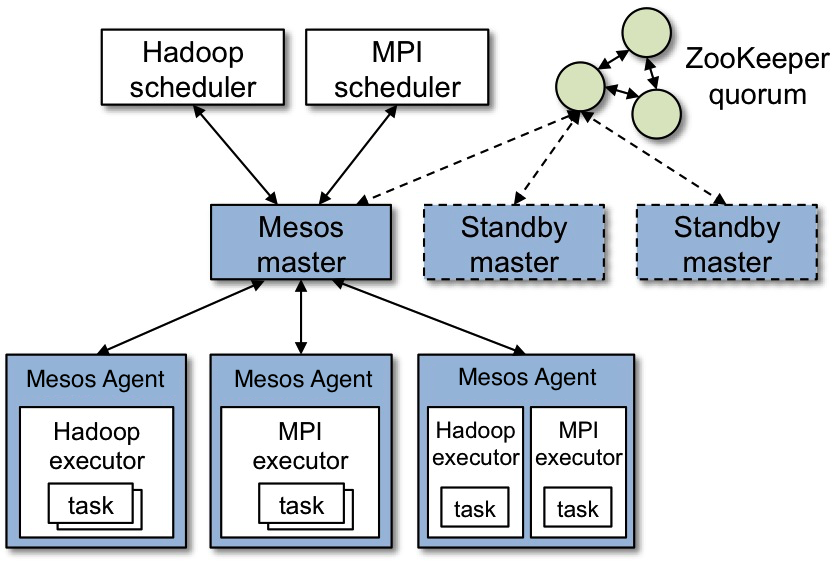
\includegraphics[width=0.6\textwidth]{images/figures/apachemesos.png}
\caption{Abstracción de nodos en Apache Mesos.\label{fig:figure_placement_example}}
\end{figure}


\section{Proveedores de Infraestructura como Servicio}

La Infraestructura como Servicio (\textit{IaaS}) es uno de los tres modelos fundamentales en el campo de la computación en la nube, junto con la Plataforma como Servicio (\textit{PaaS}) y el Software como Servicio (\textit{SaaS}). Se trata de una infraestructura informática inmediata que se aprovisiona y administra a través de una conexión pública, normalmente Internet.

Este modelo de servicio proporciona acceso a recursos informáticos situados en un entorno virtualizado, la nube. De esta manera permite reducir o escalar recursos  concretos con rapidez para ajustarlos a la demanda, pagando por uso y evitando el gasto y complejidad que suponen la compra y administración de una infraestructura física propia.

Así, existen proveedores de estos servicios informáticos en la nube que administran la infraestructura, mientras que el cliente solo tiene que configurar y administrar su propio software.

Los recursos informáticos ofrecidos consisten en hardware virtualizado o infraestructura de procesamiento. La definición de \textit{IaaS} abarca aspectos como el espacio en servidores virtuales, conexiones de red, ancho de banda, direcciones IP y balanceadores de carga. Físicamente, el repertorio de recursos hardware disponibles procede de multitud de servidores y redes, generalmente distribuidos entre numerosos centros de datos.

Entre las ventajas de \textit{IaaS} se encuentran:
\begin{itemize}
\item Eliminación del gasto en capital y corriente eléctrica.
\item Adquisición de nuevos recursos con rapidez.
\item Respuesta rápida ante cambios de demanda, aumentando y reduciendo recursos.
\item Mayor eficiencia, puesto que se garantiza que se utiliza la capacidad máxima de la infraestructura física.
\item Mayor seguridad y protección de los recursos de información.
\end{itemize}

Los ejemplos comerciales mejor conocidos son Amazon Web Services y DigitalOcean.

Por su parte, DigitalOcean, creada en 2011 por Ben y Moisey Uretsky, es un proveedor Estadounidense de servidores virtuales privados. La compañía alquila recursos de centros de cómputo existentes como Nueva York, Amsterdam, San Francisco, Londres y Singapur.

\begin{figure}[H]
\centering

\includegraphics[width=0.4\textwidth]{images/figures/digitalocean.png}
\caption{Digital Ocean.\label{fig:figure_placement_example}}
\end{figure}

Actualmente, Netcraft\footnotettt{Netcraft}{https://www.netcraft.com}, compañía de servicios de Internet orientada al análisis de mercado, ha catalogado a DigitalOcean como la segunda Compañía de alojamiento más grande del mundo, después de Amazon Web Services.

Entre sus características más destacadas está que sus servidores en la nube, llamados \textit{droplets}, pueden ser provisionados típicamente en 55 segundos. Además, provee discos duros \textit{SSD} de alto rendimiento y virtualización \textit{KVM}. En general aportan servicios mensuales por 5 dólares al mes, continuando con facturación por hora.

En la ejecución de este proyecto se aplicará el uso de Amazon Web Services como proveedor de Infraestructura como Servicio, detallado a continuación.

\subsection{Amazon Web Services}

Amazon Web Services (AWS) es una plataforma de servicios de computación en la nube ofrecida a través de Internet por Amazon.com y lanzada en 2006.

\begin{figure}[H]
\centering

\includegraphics[width=0.4\textwidth]{images/figures/aws.png}
\caption{Amazon Web Services.\label{fig:figure_placement_example}}
\end{figure}

AWS está situado en 11 Regiones geográficas: EE.UU. Este (Norte de Virginia), EE.UU. Oeste (Norte de California), EE.UU. Oeste (Oregón), AWS GovCloud (EE.UU.), São Paulo (Brasil), Irlanda, Singapur, Tokio y Sydney. Cada región está totalmente contenida dentro de un solo país y todos sus datos y servicios permanecen dentro de la región designada. Además, cada una tiene múltiples zonas de disponibilidad, diferentes centros de datos que proporcionan servicios de AWS.

Este proveedor dispone de una capa gratuita diseñada para permitir obtener experiencia práctica con los servicios en la nube de AWS. Ésta incluye 12 meses a partir de la fecha de inscripción en AWS, así como ofertas de servicios adicionales que no vencen al final de este periíodo. No obstante existen ciertos límites de uso. A partir de este primer año se empieza a pagar por horas de uso.

Ofrece una gran cantidad de recursos y servicios, innovando constantemente y creando nuevos. Concretamente, en la elaboración de este proyecto se utilizarán los servicios:

\subsubsection{AWS Identity and Access Management (IAM)}

AWS Identity and Access Management (IAM)\footnotettt{IAM}{http://docs.aws.amazon.com/es\_es/IAM/latest/UserGuide/introduction.html} es un servicio web gratuito que permite controlar de forma segura el acceso a los recursos de AWS por parte de los usuarios. Las dos principales características a usar que ofrece son el acceso compartido a la cuenta AWS concediendo permisos a otros usuarios para administrar y utilizar los recursos sin tener que compartir la clave de acceso y la concesión de permisos diferentes a distintos usuarios para diferentes recursos.

\subsubsection{Amazon Elastic Compute Cloud (Amazon EC2)}

Amazon Elastic Compute Cloud (Amazon EC2)\footnotettt{Amazon EC2}{http://docs.aws.amazon.com/es\_es/AWSEC2/latest/UserGuide/concepts.html} proporciona la capacidad de computación escalable en la nube de AWS. Su uso elimina la necesidad de invertir en hardware por adelantado, por lo que se pueden desarrollar e implementar aplicaciones más rápido. Se pueden desplegar tantos servidores virtuales como se necesite, configurar seguridad y redes y administrar el almacenamiento. Además, este servicio permite escalar o reducir los requisitos bajo demanda o picos de popularidad, reduciendo la necesidad de predecir el tráfico. La principal característica es el entorno virtual de computación o instancia. Además, ofrece otras funcionalidades como plantillas preconfiguradas, varios tipos de instancias o configuraciones de CPU, memoria, almacenamiento y capacidad de red, inicio de sesión seguro utilizando pares de claves, volúmenes de almacenamiento de datos temporales que se eliminan al detener o finalizar la instancia, múltiples ubicaciones físicas para los recursos, conocidos como regiones y zonas de disponibilidad y un firewall que permite especificar los protocolos, puertos y rangos de IP usando grupos de seguridad.

\subsubsection{Amazon Virtual Private Cloud (Amazon VPC)}

Amazon Virtual Private Cloud (Amazon VPC)\footnotettt{Amazon VPC}{http://docs.aws.amazon.com/es\_es/AmazonVPC/latest/UserGuide/VPC\_Introduction.html} permite lanzar los servicios AWS en una red virtual definida. Una nube virtual privada (VPC) es una red virtual dedicada a la cuenta de AWS. Está lógicamente aislada de otras redes virtuales en la nube AWS y permite iniciar los recursos en ella. Ésta es configurable, pudiendo seleccionar un rango de direcciones IP, crear subredes y configurar tablas de rutas, pasarelas de red y configuraciones de seguridad. Otro elemento a usar es la subred que es un rango de direcciones IP en de la VPC. Para proteger los recursos de AWS en cada subred se utilizan, entre otros, los grupos de seguridad.

\section{Otras herramientas tecnológicas}

A continuación se describirán otra serie de herramientas necesarias para la elaboración de este proyecto.

\subsection{Vagrant}

Vagrant\footnotettt{Vagrant}{https://www.vagrantup.com} es una herramienta de código abierto para crear y configurar entornos de desarrollo portátiles y virtualizados, centrada en la automatización.

\begin{figure}[H]
\centering

\includegraphics[width=0.4\textwidth]{images/figures/vagrant.png}
\caption{Vagrant.\label{fig:figure_placement_example}}
\end{figure}

Vagrant fue creada en enero de 2010 por Mitchell Hashimoto como un proyecto personal. Su primera versión fue lanzada en marzo de 2010. La primera versión estable, Vagrant 1.0, lo hizo en marzo de 2012 y, en noviembre de ese mismo año, Mitchell Hashimoto creó la organización HashiCorp para respaldar el desarrollo de Vagrant a tiempo completo, contando con la contribución de una fuerte comunidad de desarrolladores. Vagrant está escrito en lenguaje Ruby pero puede ser utilizado en proyectos escritos en otros lenguajes de programación.

La idea central detrás de su creación reside en el hecho de que el mantenimiento del entorno de desarrollo se hace cada vez más difícil a medida que el proyecto crece. De esta manera, Vagrant proporciona ambientes de trabajo menos complejos de configurar, reproducibles y portátiles.

Esta herramienta utiliza aprovisionadores y proveedores como bloques de construcción para administrar los entornos de desarrollo. Los aprovisionadores son herramientas que permiten a los usuarios personalizar la configuración de entornos virtuales, mientras que los proveedores son los servicios que Vagrant utiliza para lanzar y crear los propios entornos virtuales. Ejemplos de proveedores son VirtualBox\footnotettt{VirtualBox}{https://www.virtualbox.org}, VMWare\footnotettt{VMWare}{https://www.vmware.com/es.html}, AWS, Hyper-V\footnotettt{Hyper-V}{https://technet.microsoft.com/en-us/library/mt169373(v=ws.11).aspx}, Digital Ocean y Docker. Ejemplos de aprovisionadores son Puppet\footnotettt{Puppet}{https://puppet.com}, Chef\footnotettt{Chef}{https://www.chef.io/chef}, Ansible\footnotettt{Ansible}{https://www.ansible.com} y Shell\footnotettt{Shell}{https://www.vagrantup.com/docs/provisioning/shell.html}.

Para su puesta en marcha se utiliza un fichero de configuración denominado \kode{Vagrantfile}. Su función principal es describir el tipo de máquina requerida para un proyecto, cómo configurarla y proveerla. Por otro lado, existen cajas o \textit{boxes} que son el formato de paquetes para los ambientes Vagrant. Una caja puede ser utilizada por cualquier persona en cualquier plataforma que soporte Vagrant para crear un entorno de trabajo idéntico.

\subsection{VirtualBox}

VirtualBox es un software de virtualización de código abierto para arquitecturas x86/amd64. 

\begin{figure}[H]
\centering

\includegraphics[width=0.4\textwidth]{images/figures/virtualbox.png}
\caption{VirtualBox.\label{fig:figure_placement_example}}
\end{figure}

Este hipervisor de tipo II o \textit{hosted}, se caracteriza porque permite instalar sistemas operativos adicionales, conocidos como sistemas invitados o máquinas virtuales, dentro de otro sistema operativo, sistema anfitrión, cada uno con su propio ambiente virtual.

\begin{figure}[H]
\centering
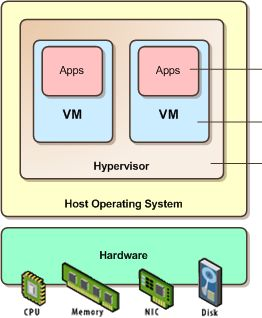
\includegraphics[width=0.4\textwidth]{images/figures/hypervisortype2.jpg}
\caption{Hipervisor tipo II.\label{fig:figure_placement_example}}
\end{figure}

VirtualBox fue creado originalmente por la empresa alemana Innotek GmbH\footnotettt{Innotek GmbH}{https://www.innotek.net} en enero de 2007. Actualmente es desarrollado por Oracle Corporation y existen dos versiones gratuitas. Por un lado la llamada Oracle VM VirtualBox, sujeta a la licencia de "Uso Personal y de Evaluación VirtualBox". Por otro lado, VirtualBox OSE, sujeta a la licencia GPL.

Entre sus características más importantes se destaca que es multiplataforma, en referencia a las arquitecturas soportadas; multi huéspedes, por la variedad y cantidad de sistemas operativos que puede virtualizar; y ofrece portabilidad, al poder importar y exportar las máquinas virtuales a otros sistemas.

\subsection{GitHub}

GitHub\footnotettt{GitHub}{https://github.com} es una plataforma de desarrollo colaborativo de software para alojar proyectos utilizando el sistema de control de versiones Git\footnotettt{Git}{https://git-scm.com}. El código se almacena de forma pública, aunque también se puede hacer de forma privada, creando una cuenta de pago.

\begin{figure}[H]
\centering

\includegraphics[width=0.4\textwidth]{images/figures/github.png}
\caption{GitHub.\label{fig:figure_placement_example}}
\end{figure}

Esta herramienta permite alojar repositorios de código y ofrece utilidades para el trabajo en equipo, dentro de un proyecto, algunas de las cuales son:
\begin{itemize}
\item Wiki: Mantenimiento de distintas versiones de páginas.
\item Sistema de seguimiento de problemas: Permite a los miembros de un equipo detallar un problema con el software o una sugerencia.
\item Visor de ramas: Permite comparar los progresos realizados en las distintas ramas del repositorio.

Además, se puede contribuir a mejorar el software de otros usuarios, a partir de la creación de programas de código abierto que fomentan el software libre.

\end{itemize}

\subsection{Travis CI}

Travis CI\footnotettt{Travis CI}{https://docs.travis-ci.com} es una compañia y sistema distribuido que ofrece servicios de Integración y Despliegue continuos (CI/CD) gratuitos o de pago.

\begin{figure}[H]
\centering

\includegraphics[width=0.4\textwidth]{images/figures/travisci.jpg}
\caption{Travis CI.\label{fig:figure_placement_example}}
\end{figure}

El servicio gratuito permite conectar el repositorio de GitHub público para poder regenerar el proyecto tras cada cambio. Así, esta herramienta fiscaliza el directorio de GitHub de manera que cuando detecta que se ha producido un cambio en él utiliza el fichero de configuración \kode{.travis.yml} para realizar las acciones descritas en el mismo. Este fichero contiene las precondiciones, condiciones y postcondiciones necesarias para construir y desplegar la aplicación en uso de manera automática. Ejemplos de dichas acciones son la comprobación de que los tests pasen satisfactoriamente, construir una nueva imagen Docker y subirla al repositorio DockerHub.

Entre los beneficios que aporta la integración continua están la reducción de riesgos y tiempo, la reducción de procesos manuales repetitivos, la obtención de una versión de software mediante un proceso conocido, confiable, probado, versionado y repetible y la mejora la visibilidad del estado del proyecto. Además, permite mantener la calidad de todo el sistema meduante la ejecución de todos los tests periódicamente, ayudando a identificar rápidamente problemas y a corregirlos antes de pasar a una versión en producción.

\subsection{Softcover}

Para la elaboración de la memoria se utiliza la gema Ruby Softcover\footnotettt{Softcover}{https://github.com/softcover/softcover} que es un sistema de composición de libros electrónicos para autores técnicos. Depende de otra gema, polytexnic\footnotettt{polytexnic}{https://github.com/skmetz/polytexnic}, para convertir la entrada de \textit{Markdown} o \textit{PolyTeX} a \textit{HTML} y \textit{LaTeX}, y de ahí a \textit{EPUB}, \textit{MOBI} y \textit{PDF}.

